\subsection{Derivate Methods}
There are again some tuned parameters in this section, see Table \ref{tab:derivative-params}.

\begin{table}[H]
\centering
  \begin{tabular}{|| c | c | c ||}
  \hline
  Flavour & Parameter & Value \\
  \hline
  \multirow{1}{*}{MultiCNN} & rgb\_layers & [32, 48, 64, 128] \\
  \hline
  \multirow{1}{*}{4-way FiLM} & downscaling\_cnn & [32, 48, 64, 128] \\
  \hline
  \multirow{3}{*}{4-way Multi View Attention} & embed\_size & 128 \\
  & num\_heads & 8 \\
  & num\_layers & 4 \\
  \hline
  \end{tabular}\caption{Default Training parameters}\label{tab:derivative-params}
\end{table}

\subsubsection{Grasp Normal}
This section
\begin{figure}[H]
  \centering
  
\includegraphics[width=\linewidth]{assets/evaluation/derivatives/grasp-normal-wd.png}
  \caption{Wrist and depth}\label{fig:deriv-normal-final-wd}
\end{figure}

\begin{figure}[H]
  \centering
  
\includegraphics[width=\linewidth]{assets/evaluation/derivatives/grasp-normal-allcams.png}
  \caption{Success rate (\%) for all modalities}\label{fig:deriv-normal-final-allcams}
\end{figure}

\begin{figure}[H]
  \centering
  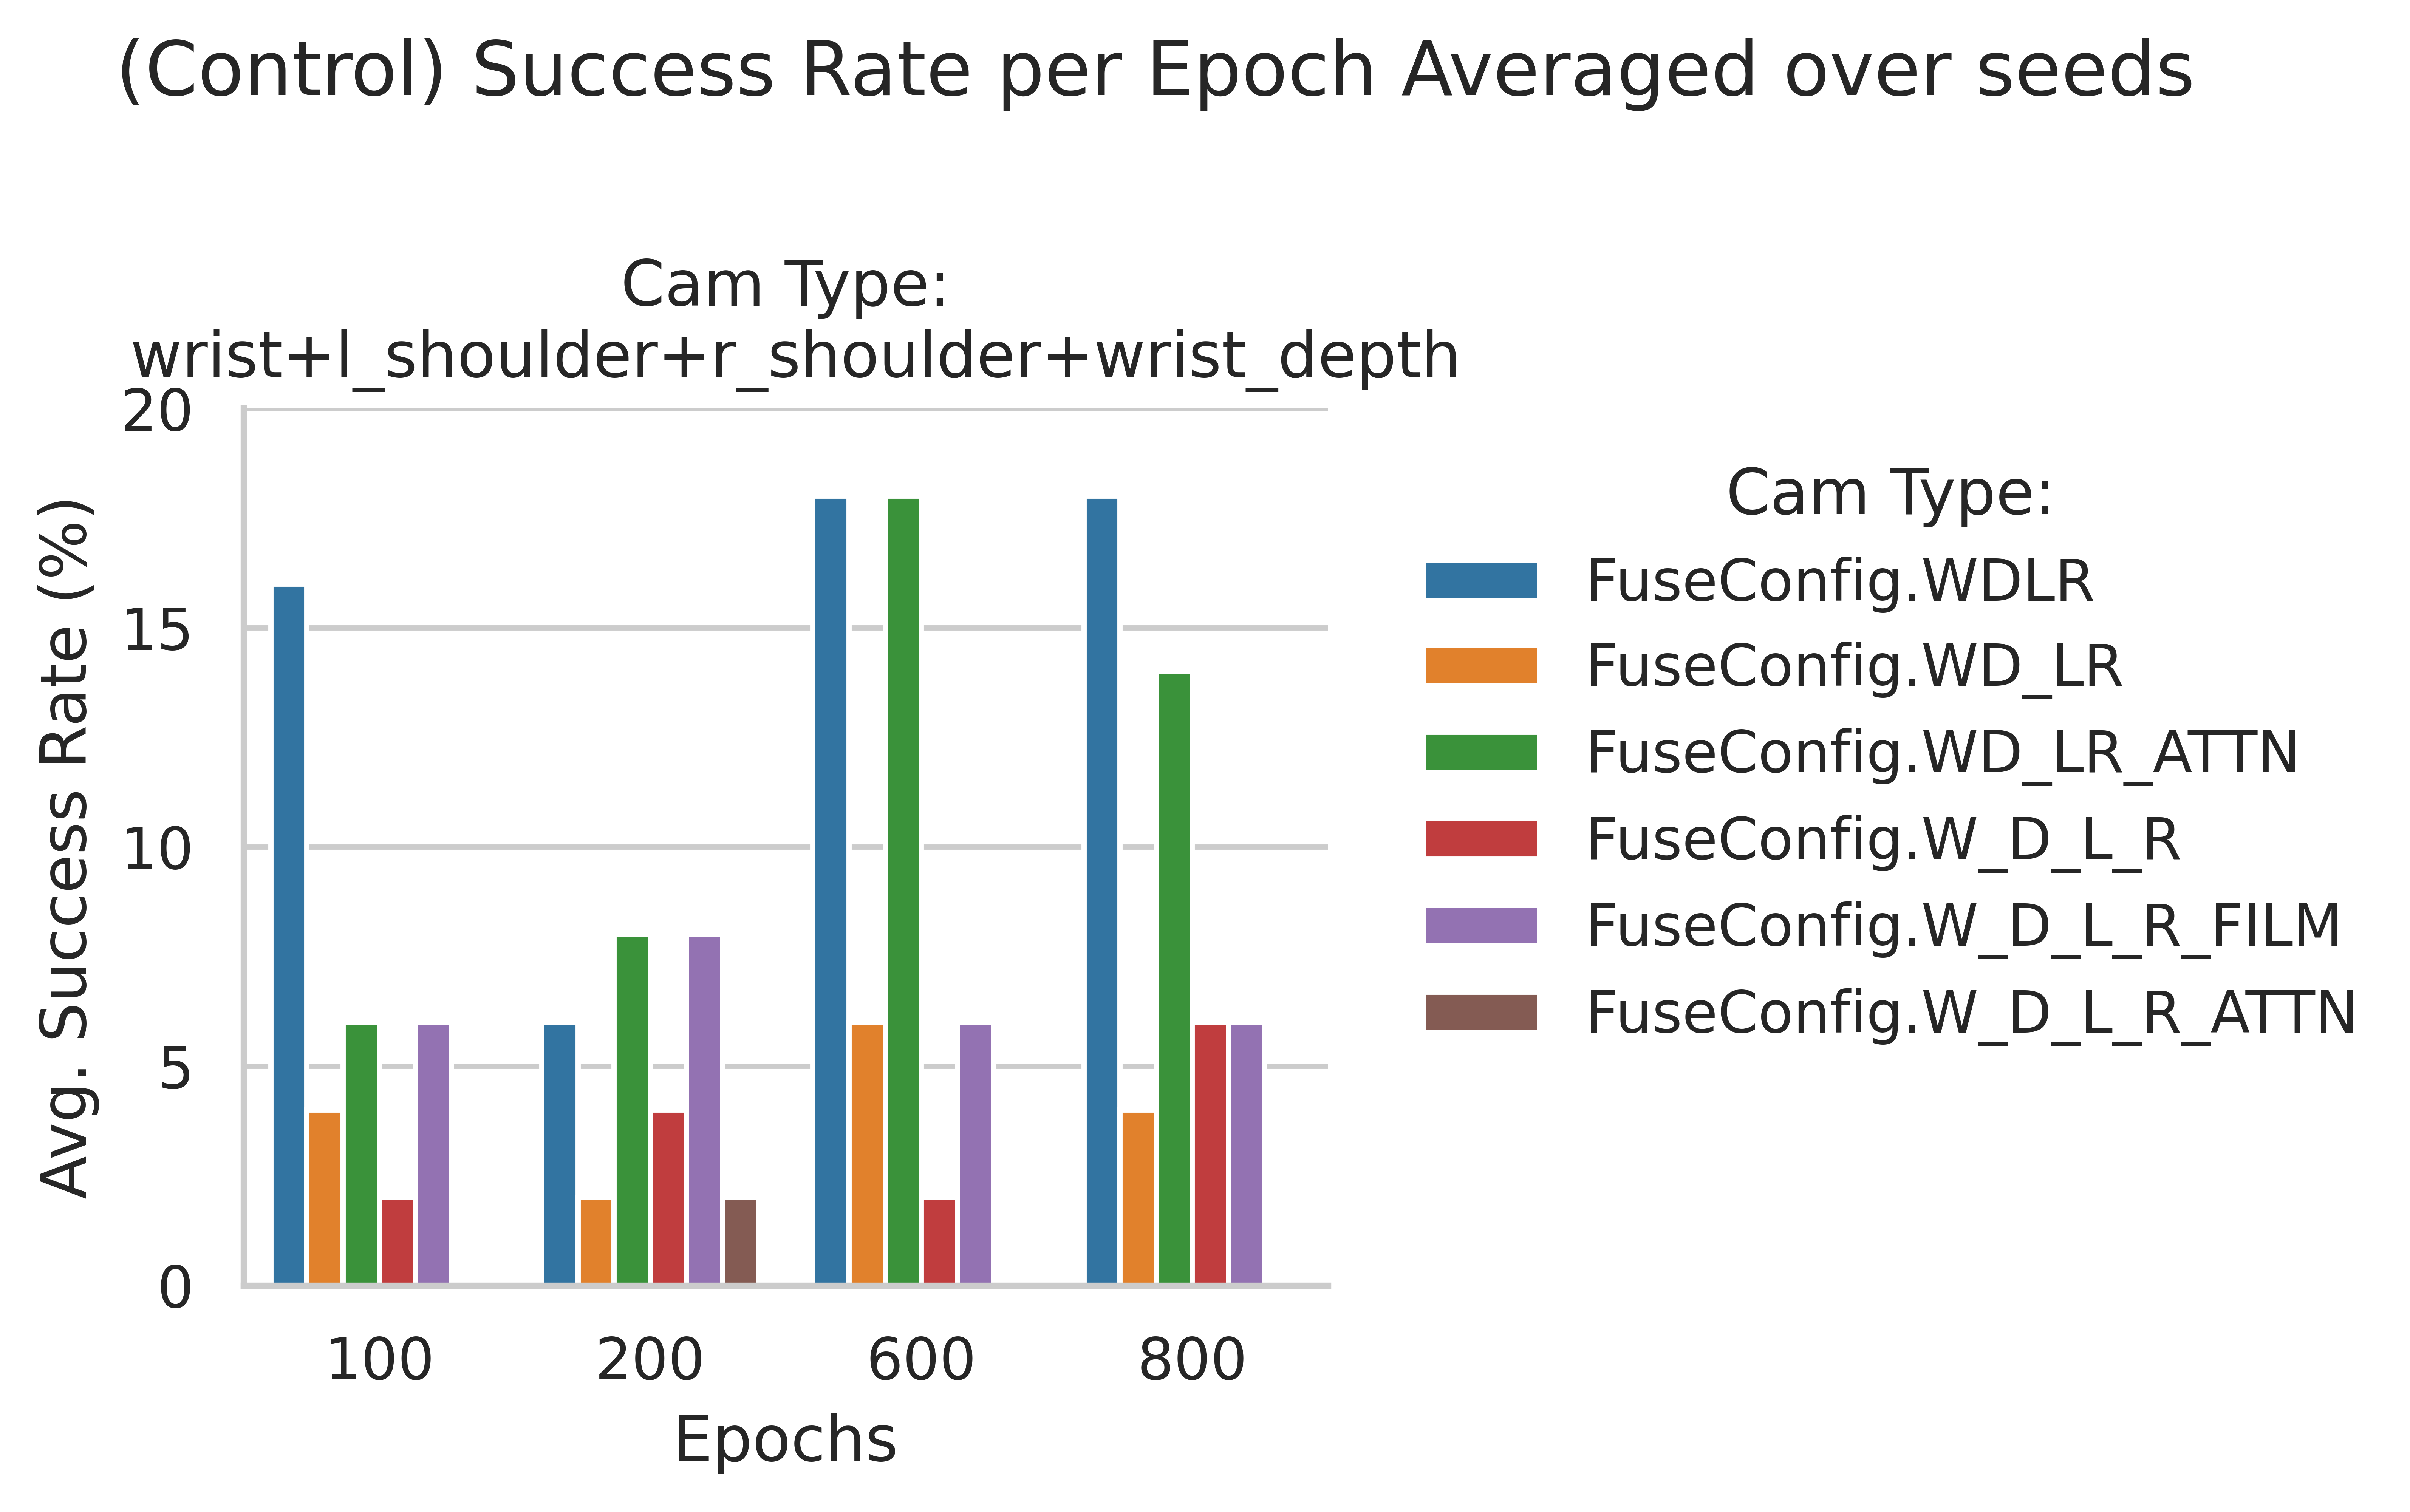
\includegraphics[width=\linewidth]{assets/evaluation/derivatives/grasp-normal-control-success-cams.png}
  \caption{Success rate (\%) for all modalities}\label{fig:derivatives-all-cams-success}
\end{figure}

There is not success for the `test' run!

\subsection{Reach}